% before-after.tex
%
% Draft section reporting the quantitative before--after static-analysis
% results (JavaParser, PMD, Checkstyle) produced under before-after/results/.
% Intended to be \input{} or merged into the main manuscript, e.g. as a
% subsection of the Discussion, or as a Supplementary robustness check
% responding to reviewer comment R5.10.
%
% Required packages (add to the main preamble if not already present):
%   \usepackage{amsmath}
%   \usepackage{booktabs}
%   \usepackage{graphicx}
% Figure paths below are relative to this file's location (before-after/);
% adjust \graphicspath or the paths themselves if this file is merged into
% a manuscript tree with a different layout.
%
% All figures reported here are read directly from the CSV/JSON outputs of
% JavaParser_Before_After_Analysis(_Readable).ipynb, PMD_Before_After_Analysis.ipynb,
% and Checkstyle_Before_After_Analysis.ipynb; no additional computation was
% performed to produce this section.
%
% Reproducibility note: pandas/scipy/matplotlib are pinned to exact
% versions (2.3.3/1.13.1/3.9.4) in all four notebooks as of this revision.
% An earlier, unpinned run produced a different JavaParser abrupt-exit-count
% p-value (0.047 vs. the pinned 0.061) for the identical Wilcoxon statistic,
% because scipy.stats.wilcoxon(method="auto") can silently choose a
% different p-value approximation across environments. All figures below
% reflect the pinned, reproducible configuration.

\section{Quantitative Before--After Robustness Check}
\label{sec:before-after-robustness}

To address the concern that the manuscript presents descriptive
observations rather than strong empirical evidence that the proposed
method consistently improves software quality (reviewer comment R5.10), we
conducted a paired, multi-measure static-analysis comparison of every
original Stack Overflow snippet against its most recent revision, for the
125 unique, dataset-eligible before--after histories whose \emph{Final
Manual Validation} value is \texttt{Agress Yes}. Three independent tools
were used, each targeting a distinct quality dimension: JavaParser for
intrinsic AST-based structural measures, a reduced PMD ruleset for
bug-risk and performance indicators, and a reduced Checkstyle
configuration for readability. Each pair was tried under three
symmetric wrapper strategies (raw source, class-member, method-body) and
analyzed only when both the original and the revised snippet shared a
common successful parse mode. Full methodological detail is given in
Section~\ref{sec:methodology}\footnote{Cross-reference to be updated to
the manuscript's Methodology section on merge.}.

\subsection{Parsing coverage}
\label{sec:before-after-coverage}

Table~\ref{tab:ba-coverage} summarizes how many of the 125 scoped pairs
each tool was able to analyze. All three tools independently exclude
roughly a third of the scoped sample because the original and the latest
snippet never shared a common successful parse mode -- consistent
exclusion rates across three independently implemented extractors suggest
this reflects a genuine property of the snippets (fragments that only
parse under one specific wrapper on one side of the pair) rather than a
defect in any single tool.

\begin{table}[htbp]
\centering
\caption{Parsing coverage of the 125 scoped \texttt{Agress Yes} pairs, by
tool.}
\label{tab:ba-coverage}
\begin{tabular}{lrrrr}
\toprule
Tool & Scoped pairs & Analyzed & Excluded & Exclusion rate \\
\midrule
JavaParser            & 125 & 80 & 45 & 36.0\% \\
PMD (reduced ruleset) & 125 & 77 & 48 & 38.4\% \\
Checkstyle            & 125 & 81 & 44 & 35.2\% \\
\bottomrule
\end{tabular}
\end{table}

\begin{table}[htbp]
\centering
\caption{Wrapper mode under which analyzed pairs achieved a common
successful parse.}
\label{tab:ba-parse-mode}
\begin{tabular}{lrrr}
\toprule
Tool & \textsc{raw} & \textsc{class\_member} & \textsc{method\_body} \\
\midrule
JavaParser & 66 & 5  & 9 \\
PMD        & 21 & 47 & 9 \\
Checkstyle & 70 & 2  & 9 \\
\bottomrule
\end{tabular}
\end{table}

JavaParser and Checkstyle predominantly succeed under the raw-source
mode, whereas PMD requires the class-member wrapper for the majority of
its analyzed pairs (47/77). We attribute this to PMD's parser being less
tolerant of top-level code fragments than JavaParser's parser or
Checkstyle's checks, rather than to any difference in the underlying
snippets, since all three tools draw from the same 125-pair manifest and
identical wrapper text.

\subsection{Structural metrics (JavaParser)}
\label{sec:before-after-javaparser}

Eighteen structural metrics (method, parameter, and local-variable
counts; branch, loop, and switch counts; a documented
cyclomatic-complexity proxy; maximum control-flow nesting; abrupt exits;
try/resource-handling counts; null-comparison counts; and an aggregate
exception-handling count) plus non-comment code-line count were each
tested independently via a paired Wilcoxon signed-rank test, with Holm's
step-down procedure applied across all 19 tests to control the
family-wise error rate. Table~\ref{tab:ba-javaparser} reports the full
results for the $n=80$ analyzed pairs.

Alongside each Wilcoxon test, a matched-pairs rank-biserial correlation
is reported as a signed effect size (after minus before): positive values
indicate the after distribution is stochastically larger, negative values
that it is stochastically smaller.

\begin{table}[htbp]
\centering
\caption{Paired JavaParser structural-metric comparison ($n=80$).
\emph{Dec.}/\emph{Unc.}/\emph{Inc.} denote the number of pairs whose
metric decreased, was unchanged, or increased from the original to the
latest revision. $p$ is the raw two-sided Wilcoxon signed-rank
$p$-value; $r_{\text{rb}}$ is the matched-pairs rank-biserial correlation
(after $-$ before); $p_{\text{Holm}}$ is Holm-corrected across all 19
metrics. No metric is significant at $\alpha=0.05$ after correction.}
\label{tab:ba-javaparser}
\small
\begin{tabular}{lrrrrrrr}
\toprule
Metric & $\Delta$ median & Dec. & Unc. & Inc. & $p$ & $r_{\text{rb}}$ & $p_{\text{Holm}}$ \\
\midrule
Code lines                & $+1$ & 19 & 19 & 42 & 0.015 & $+0.357$ & 0.273 \\
Method count               & $0$  & 7  & 58 & 15 & 0.321  & $+0.253$ & 1.000 \\
Parameter count             & $0$  & 8  & 62 & 10 & 0.442  & $+0.216$ & 1.000 \\
Max.\ parameters            & $0$  & 5  & 71 & 4  & 1.000  & $0.000$ & 1.000 \\
Local-variable count        & $0$  & 8  & 54 & 18 & 0.116  & $+0.356$ & 1.000 \\
\texttt{if} count            & $0$  & 9  & 62 & 9  & 0.766  & $-0.088$ & 1.000 \\
Loop count                  & $0$  & 0  & 78 & 2  & 0.500  & $+1.000$ & 1.000 \\
Switch count                 & $0$  & 0  & 80 & 0  & --     & --  & --    \\
Catch count                  & $0$  & 3  & 71 & 6  & 0.426  & $+0.333$ & 1.000 \\
Cyclomatic-complexity proxy  & $0$  & 10 & 53 & 17 & 0.336  & $+0.220$ & 1.000 \\
Max.\ control nesting        & $0$  & 7  & 66 & 7  & 0.542  & $+0.200$ & 1.000 \\
Abrupt-exit count            & $0$  & 7  & 57 & 16 & 0.061 & $+0.449$ & 1.000 \\
Try count                    & $0$  & 2  & 71 & 7  & 0.129  & $+0.600$ & 1.000 \\
Try-with-resources count     & $0$  & 0  & 79 & 1  & 1.000  & $+1.000$ & 1.000 \\
Throw count                  & $0$  & 1  & 74 & 5  & 0.438  & $+0.429$ & 1.000 \\
Empty-catch count            & $0$  & 1  & 76 & 3  & 0.625  & $+0.500$ & 1.000 \\
Empty-block count            & $0$  & 2  & 75 & 3  & 0.813  & $+0.200$ & 1.000 \\
Null-check count             & $0$  & 5  & 73 & 2  & 0.375  & $-0.393$ & 1.000 \\
Exception-handling count     & $0$  & 4  & 66 & 10 & 0.153  & $+0.457$ & 1.000 \\
\bottomrule
\end{tabular}
\end{table}

For nearly every metric, the majority of pairs are unchanged (e.g.\
switch count: 80/80; method count: 58/80; cyclomatic-complexity proxy:
53/80), indicating that most revisions do not alter the snippet's
structural shape. The only metric with a raw $p<0.05$ is code-line count
($p=0.015$), which increases in 42 of 80 pairs (median $\Delta=+1$
line) -- consistent with the interpretation that revisions more often
\emph{add} code (e.g.\ validation or defensive checks) than remove it --
but this does not survive Holm correction ($p_{\text{Holm}}=0.273$). No
structural metric is statistically significant after correction.

Several of the largest-looking rank-biserial values (loop count $+1.00$,
try-with-resources count $+1.00$, try count $+0.60$, empty-catch count
$+0.50$) come from metrics with only 1--9 nonzero-delta pairs out of 80.
An effect size computed from one or two nonzero pairs is not a meaningful
estimate -- it is a symptom of severe underpowering for that metric, not
evidence of a competing large effect alongside code-line count.

Within the Bug Fixing subgroup ($n=12$), code-line count shows a raw
$p=0.039$ (7/12 pairs increased); within Improving Code ($n=65$), the
same metric gives $p=0.099$ (33/65 increased). Both subgroup results are
uncorrected and exploratory; every other structural metric in both
subgroups is dominated by unchanged pairs and shows no separation from
the null.

\subsection{Bug-risk and performance violations (PMD)}
\label{sec:before-after-pmd}

The reduced PMD ruleset (12 bug-risk rules, 7 performance rules) is
sparse at the snippet level: across the $n=77$ analyzed pairs, only 81
violations were retained in total (72 bug-risk, 9 performance), across
\emph{both} versions combined. Table~\ref{tab:ba-pmd} reports paired
Wilcoxon tests and rank-biserial effect sizes for raw violation counts
and violations per 100 non-comment lines, separately for the combined
ruleset, the bug-risk subset, and the performance subset.

\begin{table}[htbp]
\centering
\caption{Paired PMD violation comparison ($n=77$). Rank-biserial
correlation is signed after $-$ before; a negative value indicates the
after distribution is stochastically smaller (i.e.\ fewer violations).
$p_{\text{Holm}}$ is Holm-corrected across all six rows. No result is
significant at $\alpha=0.05$.}
\label{tab:ba-pmd}
\small
\begin{tabular}{llrrrrrrr}
\toprule
Dimension & Metric & Imp. & Unc. & Wors. & $p$ & Rank-biserial & $p_{\text{Holm}}$ \\
\midrule
Combined     & Raw violations         & 5  & 66 & 6 & 0.520 & $+0.24$ & 1.000 \\
Combined     & Violations / 100 lines & 16 & 52 & 9 & 0.578 & $-0.13$ & 1.000 \\
Bug-risk     & Raw violations         & 5  & 67 & 5 & 0.695 & $+0.18$ & 1.000 \\
Bug-risk     & Violations / 100 lines & 14 & 55 & 8 & 0.588 & $-0.14$ & 1.000 \\
Performance  & Raw violations         & 0  & 76 & 1 & 1.000 & $+1.00$ & 1.000 \\
Performance  & Violations / 100 lines & 3  & 73 & 1 & 0.875 & $-0.20$ & 1.000 \\
\bottomrule
\end{tabular}
\end{table}

No PMD metric approaches significance. The per-100-line density measures
lean mildly toward improvement in both the combined and bug-risk
dimensions (more improved than worsened pairs), but the corresponding
raw-count results are close to a wash (e.g.\ 5 improved vs.\ 6 worsened,
combined). Because density can decrease simply because a revision adds
lines, without any violation being fixed, we consider the raw-count
result the more conservative and more informative of the two.

Table~\ref{tab:ba-pmd-rules} lists the PMD rules with any observed
before/after activity (rules with zero removed and zero introduced
instances across all pairs are omitted).

\begin{table}[htbp]
\centering
\caption{PMD rule-level transitions with nonzero activity. Net removed
= removed $-$ introduced; positive values indicate net improvement.}
\label{tab:ba-pmd-rules}
\small
\begin{tabular}{llrrrr}
\toprule
Rule & Dimension & Removed & Introduced & Preserved & Net removed \\
\midrule
\texttt{AssignmentInOperand}             & Bug-risk    & 3 & 1 & 7 & $+2$ \\
\texttt{IdenticalCatchBranches}          & Bug-risk    & 1 & 1 & 1 & $0$ \\
\texttt{UseStringBufferForStringAppends} & Performance & 1 & 1 & 1 & $0$ \\
\texttt{AppendCharacterWithChar}         & Performance & 0 & 1 & 1 & $-1$ \\
\texttt{CompareObjectsWithEquals}        & Bug-risk    & 0 & 1 & 0 & $-1$ \\
\texttt{EmptyCatchBlock}                 & Bug-risk    & 0 & 1 & 7 & $-1$ \\
\bottomrule
\end{tabular}
\end{table}

Two resource-leak rules central to the Fixing Bug narrative,
\texttt{CloseResource} and \texttt{UseTryWithResources}, show zero
removed and zero introduced instances (omitted from
Table~\ref{tab:ba-pmd-rules}); every occurrence present was already
present in both versions. \texttt{EmptyCatchBlock} and
\texttt{CompareObjectsWithEquals} each show one pair in which a
revision \emph{introduced} a new violation with none removed elsewhere
-- at least one latest-version snippet in this sample is, by this
specific rule, worse than the original it replaces.

Within the Bug Fixing subgroup ($n=11$), the bug-risk dimension shows 0
improved, 10 unchanged, and 1 worsened pair ($p=1.000$); within Improving
Code ($n=63$), 5 improved, 55 unchanged, 3 worsened ($p=0.844$). The
Bug Fixing result is driven largely by the fact that 10 of 11 pairs have
zero bug-risk violations on \emph{both} sides -- there is little for a
fix to remove under this deliberately narrow, conservative ruleset, and
this analysis should not be read as evidence against the value of those
fixes.

\subsection{Readability (Checkstyle)}
\label{sec:before-after-checkstyle}

Eight readability/style checks were applied to the $n=81$ analyzed
pairs, yielding 844 retained findings in total.
Table~\ref{tab:ba-checkstyle} reports the paired comparison.

\begin{table}[htbp]
\centering
\caption{Paired Checkstyle finding comparison ($n=81$). $p_{\text{Holm}}$
is Holm-corrected across both rows. No result is significant at
$\alpha=0.05$.}
\label{tab:ba-checkstyle}
\small
\begin{tabular}{lrrrrrr}
\toprule
Metric & Imp. & Unc. & Wors. & $p$ & Rank-biserial & $p_{\text{Holm}}$ \\
\midrule
Raw findings         & 14 & 55 & 12 & 0.452 & $-0.17$ & 0.723 \\
Findings / 100 lines & 23 & 44 & 14 & 0.362 & $-0.17$ & 0.723 \\
\bottomrule
\end{tabular}
\end{table}

The density measure shows the largest directional lean of the three
tools (23 improved vs.\ 14 worsened pairs), though still far from
significant. Table~\ref{tab:ba-checkstyle-rules} shows the checks with
nonzero before/after activity.

\begin{table}[htbp]
\centering
\caption{Checkstyle rule-level transitions with nonzero activity.}
\label{tab:ba-checkstyle-rules}
\small
\begin{tabular}{lrrrr}
\toprule
Check & Removed & Introduced & Preserved & Net removed \\
\midrule
\texttt{FileTabCharacter}                  & 4 & 3 & 18 & $+1$ \\
\texttt{OneStatementPerLine}                & 1 & 1 & 0  & $0$ \\
\texttt{MultipleVariableDeclarations}       & 0 & 1 & 2  & $-1$ \\
\texttt{VariableDeclarationUsageDistance}   & 0 & 1 & 1  & $-1$ \\
\texttt{LineLength}                          & 0 & 2 & 5  & $-2$ \\
\texttt{NeedBraces}                          & 0 & 2 & 17 & $-2$ \\
\bottomrule
\end{tabular}
\end{table}

\texttt{FileTabCharacter} is the only check with a net improvement.
\texttt{LineLength} and \texttt{NeedBraces} each show two revisions
introducing a new violation with none fixed; \texttt{NeedBraces} also has
the largest \emph{preserved} count (17), indicating most brace-omission
issues present in the original snippet are simply carried over unchanged
rather than addressed. Within subgroups, Bug Fixing ($n=12$) shows 2
improved and 2 worsened pairs ($p=0.875$); Improving Code ($n=66$) shows
10 improved and 10 worsened ($p=0.430$) -- both exactly balanced, with no
directional signal.

\subsection{Cross-tool synthesis}
\label{sec:before-after-synthesis}

Across all three independently implemented dimensions -- structural
(JavaParser), bug-risk and performance (PMD), and readability
(Checkstyle) -- no metric reaches statistical significance after
appropriate correction, in either the full analyzed sample or the Bug
Fixing / Improving Code subgroups. Where a directional lean exists, it is
(i) small in magnitude where estimable with reasonable power (rank-biserial
correlations under $0.25$ in absolute value for PMD and Checkstyle
throughout; JavaParser's estimates reach $\pm0.6$ only for metrics with
as few as 1--2 nonzero-delta pairs, an artifact of a tiny effective
sample rather than evidence of a real large effect); (ii) more pronounced
in per-100-line density
measures than in raw counts, consistent with a denominator effect from
revisions adding lines rather than with violations being fixed; and
(iii) mixed at the individual rule level, with specific rules trending
worse (\texttt{EmptyCatchBlock}, \texttt{CompareObjectsWithEquals},
\texttt{LineLength}, \texttt{NeedBraces}) even as the aggregate leans
positive. With $n=77$--$81$ analyzed pairs and frequently single-digit
improved/worsened counts, particularly for the sparse PMD ruleset, these
tests are underpowered for anything short of a large effect; the
absence of significance is consistent with limited statistical power as
much as with the absence of a true effect, and we report it as such
rather than as proof of no improvement.

\subsection{Implications}
\label{sec:before-after-implications}

This quantitative analysis, taken alone, does not provide strong
statistically significant evidence that recent Stack Overflow revisions
consistently improve static-analysis indicators of software quality. It
is best read as a pre-registered robustness check that appropriately
tempers, rather than substitutes for, the manuscript's primary evidence
for the improvement claim: the manual classification of 391 applicable
recommendations (57 Fixing Bug, 334 Improving Code) and the practical
validation via pull request acceptance (11 of 36 Fixing Bug
recommendations merged into real open-source projects). We revise our
claim accordingly: compared with their original versions, recent Stack
Overflow revisions show small, non-significant, and rule-dependent
changes in static-analysis indicators of maintainability, bug-risk, and
readability, with directional trends leaning toward improvement in
violation density but not in raw counts, and with the strongest,
independently validated evidence for improvement coming from manual
classification and practical pull-request acceptance rather than from
paired static-analysis metrics alone.

% Optional supporting figures (uncomment and adjust paths/packages as needed):
% \begin{figure}[htbp]
%   \centering
%   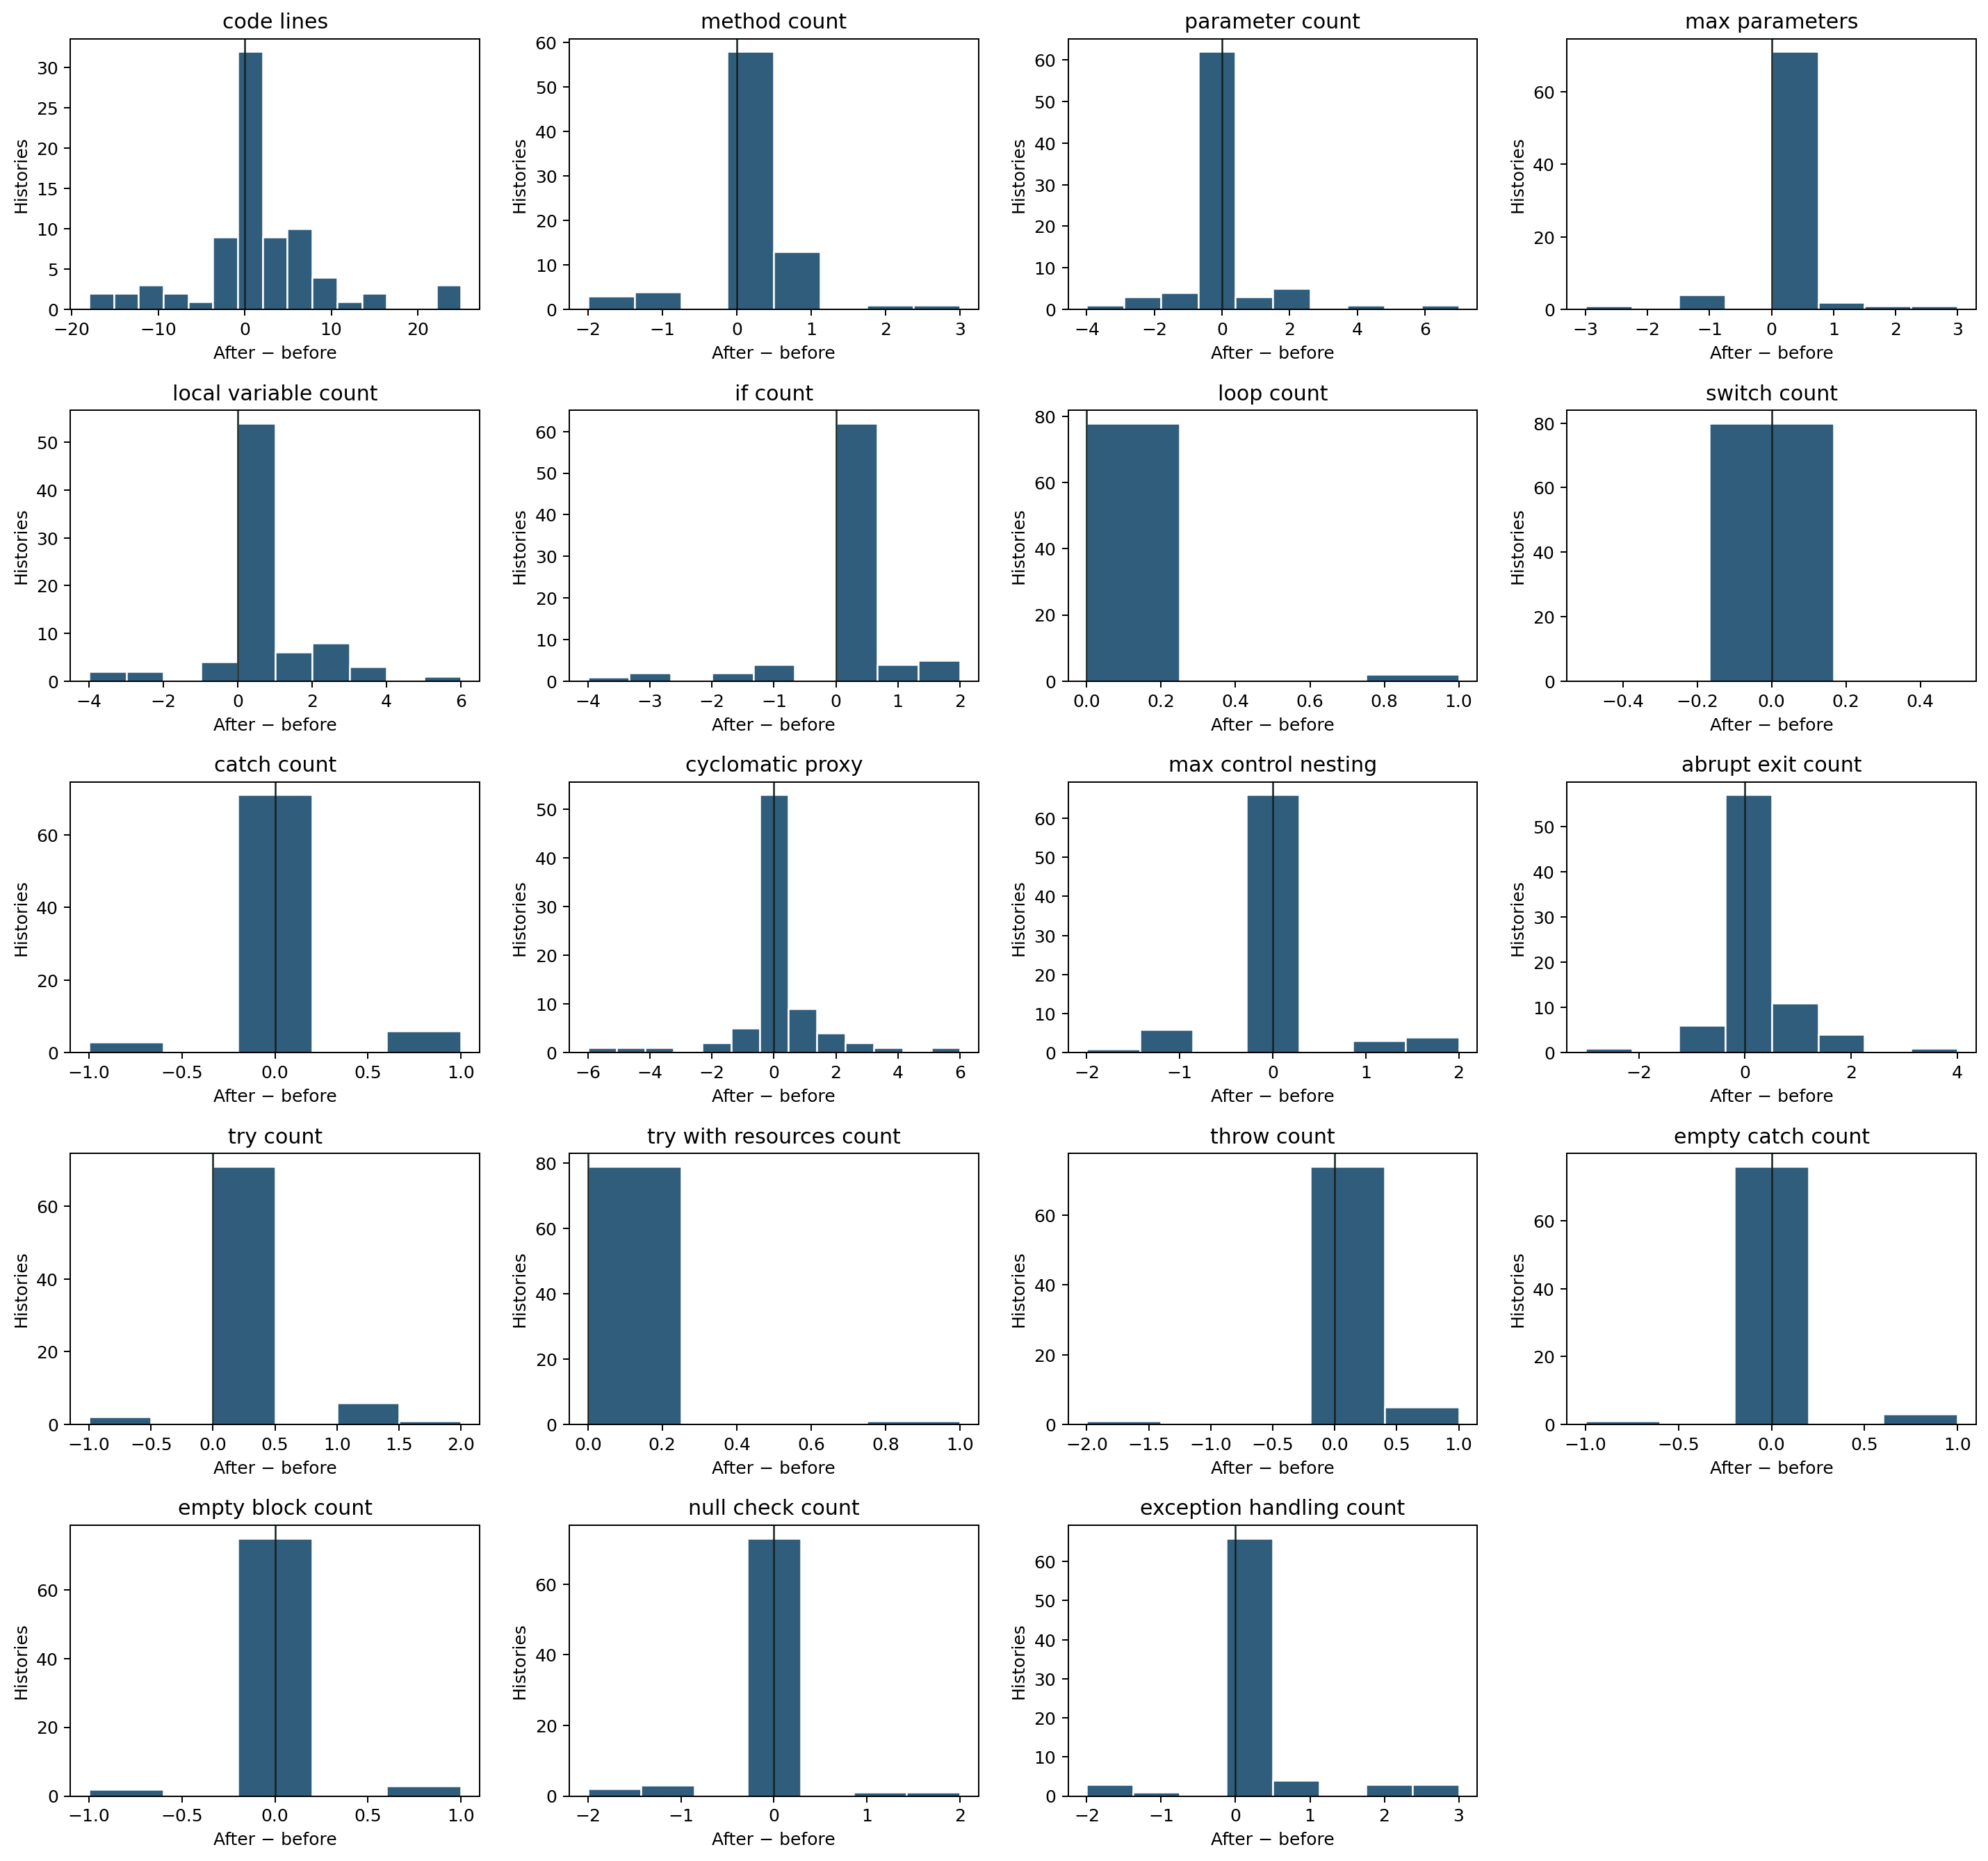
\includegraphics[width=0.95\linewidth]{results/javaparser_readable/javaparser_metric_deltas.png}
%   \caption{Distribution of after$-$before deltas for all 19 JavaParser
%   structural metrics ($n=80$ analyzed pairs).}
%   \label{fig:ba-javaparser-deltas}
% \end{figure}
% \begin{figure}[htbp]
%   \centering
%   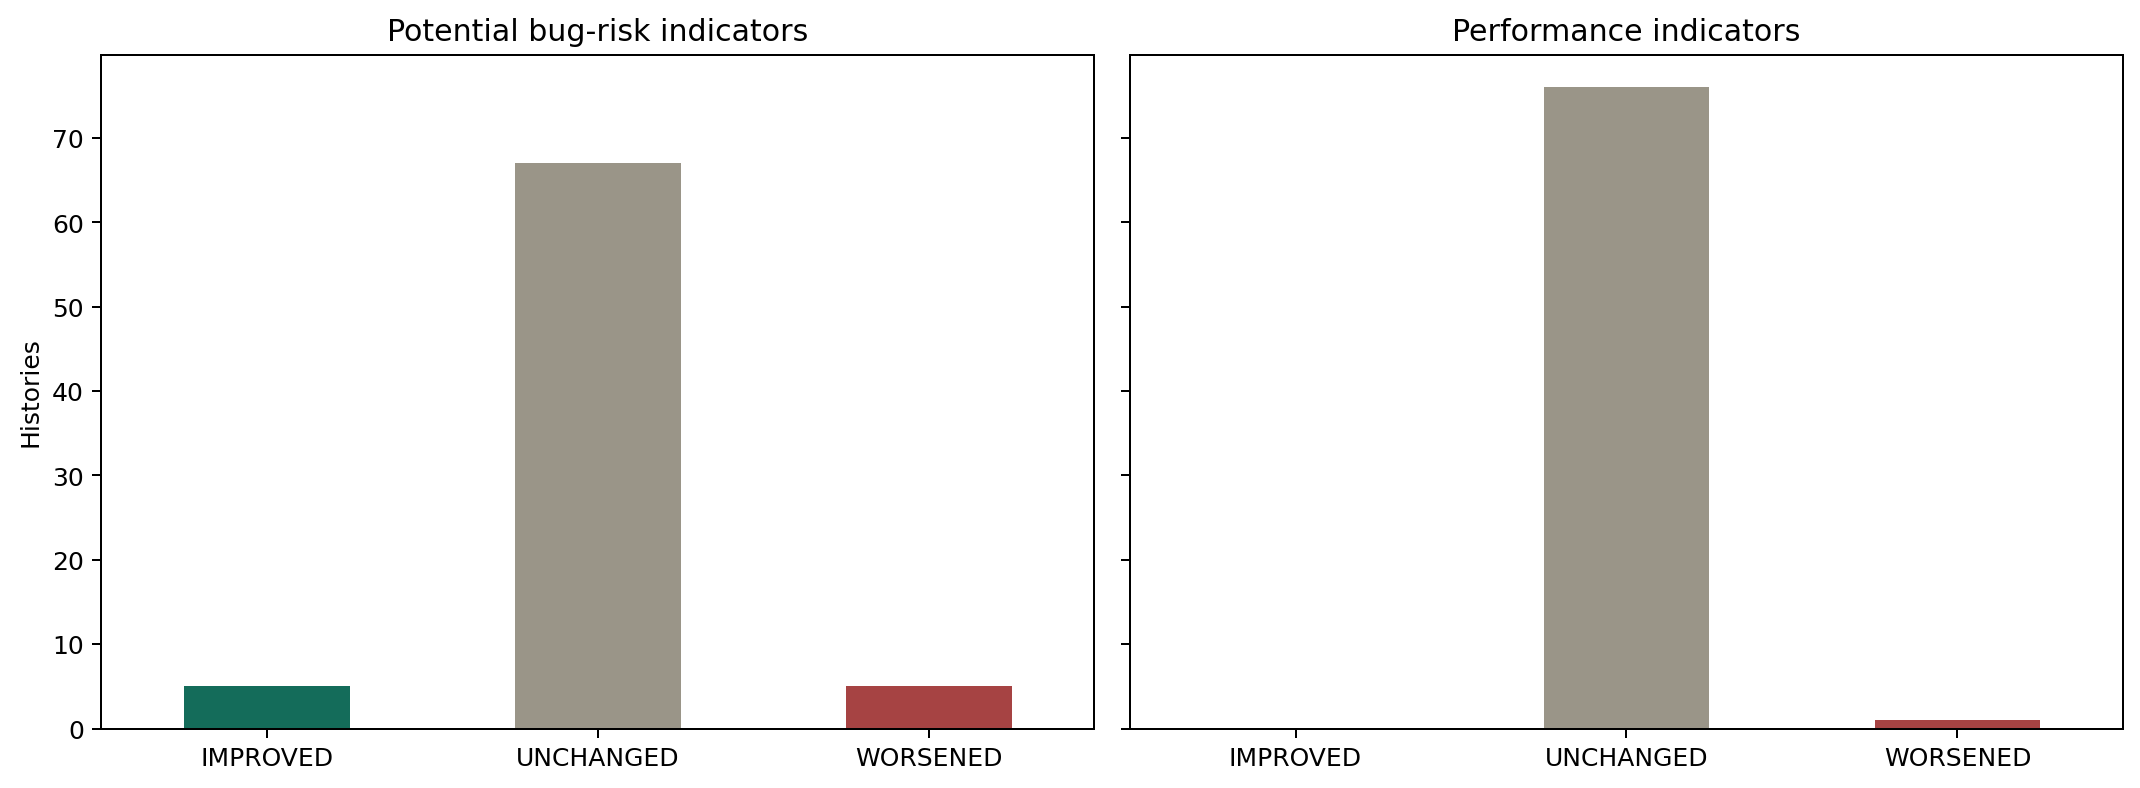
\includegraphics[width=0.95\linewidth]{results/pmd_reduced/pmd_reduced_outcomes.png}
%   \caption{PMD reduced-ruleset before--after outcomes ($n=77$ analyzed pairs).}
%   \label{fig:ba-pmd-outcomes}
% \end{figure}
% \begin{figure}[htbp]
%   \centering
%   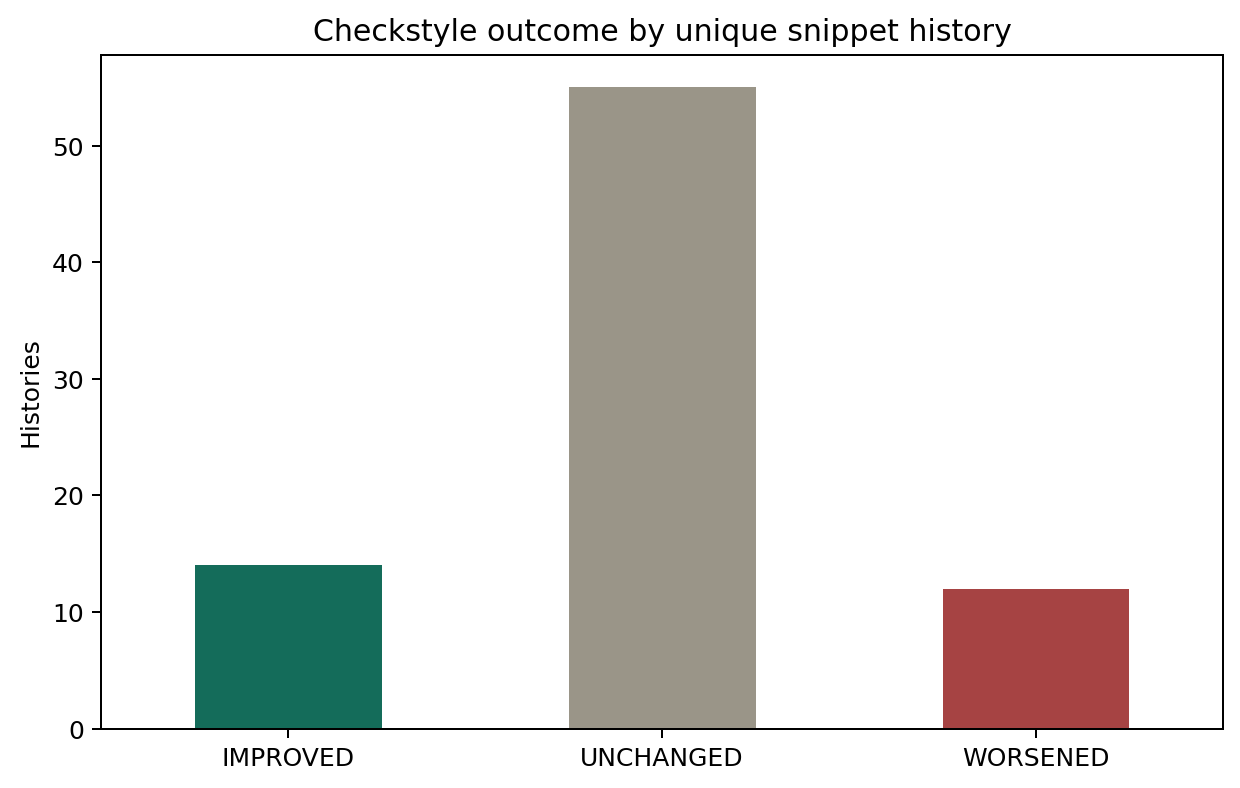
\includegraphics[width=0.95\linewidth]{results/checkstyle/checkstyle_outcomes.png}
%   \caption{Checkstyle before--after outcomes ($n=81$ analyzed pairs).}
%   \label{fig:ba-checkstyle-outcomes}
% \end{figure}
